%% Dit is de domeinanalyse: Composite Objects %%
%% Freek 26 september: Een derde domeinanalyse zou kunnen gaan over hoe om te
%% gaan met Composite objects (bijv. hoe grafisch weer te geven, hoe op te
%% slaan in de data structuur)

\documentclass[a4paper,11pt,final]{article}

\usepackage[english]{babel}
\usepackage{graphicx}
\usepackage{hyperref}
\hypersetup{ colorlinks = true, citecolor = blue,linkcolor = blue }
\usepackage[a4paper]{geometry}
\usepackage{titlesec}% added to change section headers, see newcommand definition.


\bibliographystyle{alpha}

		

\begin{document}
\selectlanguage{english}
\begin{titlepage}
	\vspace*{\fill}
	\begin{center}
		\textsc{\large WickedXmas Domain Analysis}\\[0.5cm]
		\textsc{\huge Composite Objects}\\[0.5cm]
		\textsc{Stefan Versluys}\\ \textsc{\scriptsize 19/10/2014}\\[2.0cm]
		
\includegraphics[width=0.25\textwidth]{wXm}
	\end{center}
	\vspace*{\fill}
\end{titlepage}


\tableofcontents

\newpage

\section{Introduction}
\paragraph{}
This domain analysis concerns composite objects,
along with primitive objects this kind of objects can be used to design xMAS
models with the WickedXmas tool. In fact composite objects are xMAS models
itself but left open with connection points, parameterizable and allow reuse.
The benefits of composite objects are those of reusability, it makes complex
things look simple and maintainable, it preserves correctness.

When designing an xMAS model in WickedXmas, the designer can make use of
composite objects similar as he or she does with primitive objects. Because
composite objects are xMAS models these can be edited just as any other kind
of xMAS model except that there are connection points as mentioned before.

\paragraph{}
In the next section you'll find a briefly description of the WickedXmas tool,
so you'll get an idea of how composite objects are managed and (re)used.
After that there's a description of the properties from primitive objects
followed by these of composite objects.
How models are stored as persistent data structures will be discussed in
the JSON section.

To finalise you'll find a domain example out of an other kind of industry but
who had the same reason to build a graphical design tool and with a lot of
similarities.
Especially the management and facilities of reusable objects is an 
interesting topic which can inspire future designers or users of the
WickedXmas tool.

\newpage
\section{WickedXmas}
In this section I'll briefly describe the WickedXmas tool which is used
to create, edit, view or verify xMAS models. Secondly I will show how
composite objects are created and used in this tool.
WickedXmas saves models as json formatted files which have "wck" as
extension. The same holds for composite objects with some minor
differences. Models can be made of primitive objects and composite objects,
to visualise models, objects have graphical properties along with some
specific properties. 
This document only concerns the properties necessary to represent an
xMAS model so it can be visualised,edited, stored and exchanged with
the verification interface.

\begin{figure}[here]
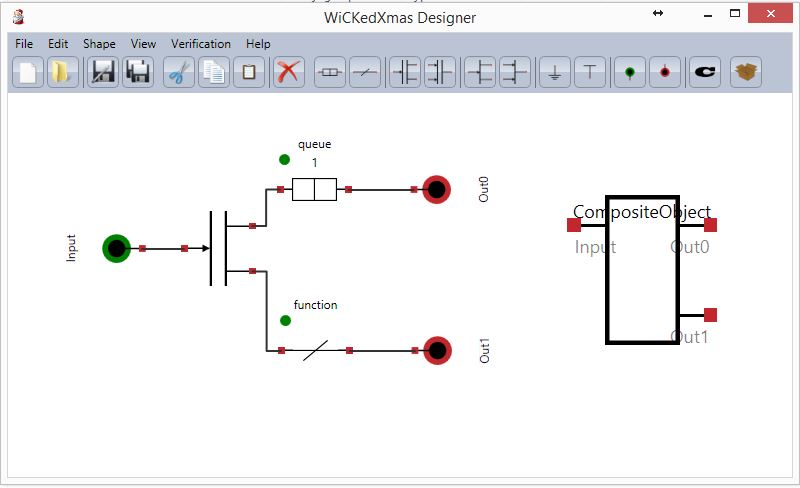
\includegraphics[width=1.0\textwidth]{wxmCO}
\caption{WickedXmas Tool and Composite objects}
\label{fig:wxmCO}
\end{figure}
Figure~\ref{fig:wxmCO} shows us the WickedXmas tool visualising the contents
of "CompositeObject.wck". At the left side we see that this is a composite
object because of the connection points. At the right side you see how this 
composite object is visualised when it is reused.

The toolbar has several buttons, eight of these are used to draw
primitive objects which are discussed in the next section. You can recognise
these by the pictogram in the button. Then two other buttons are used to
draw an input or output connection point followed by a big ``C'' button
used to add a composite object for reuse.
The button with the open box image opens the packet configuration
window where a user can add fields with their ranges. These fields can be
used into the function property of some objects.


\newpage
\section{Primitive objects}
Primitive objects are the base of xMAS models and so they do for composite
objects, so primitives determine the underlying structures of these.
Secondly, when using composite objects to create a model, there are a lot of
similarities with primitive objects. Given this knowledge we can say that
we can not ignore primitive objects in a context of composite objects, so
primitive objects need some kind of explanation.

The xMAS language has only eight primitive objects,
each object has a visual representation and one or more properties which can be
changed during modelling. Some of these properties requires a valid
value otherwise a visual marker, shown as a dot as part of the object, will lit up red instead of
green. Finally all objects have one or more ports and can be of input or output
type. The graphical representation of a port is a red filled square. 
To form a valid channel, each port must be wired to exactly one
opposite port type of an other object.

\paragraph{Common properties:}
\begin{itemize}
\item Label: A string which tags the object.
\item Position: x and y-coordinates where the object is drawn on screen.
\item Orientation: A value that represents the direction in which the object is drawn on screen.
\end{itemize}

\subsection{Queue}
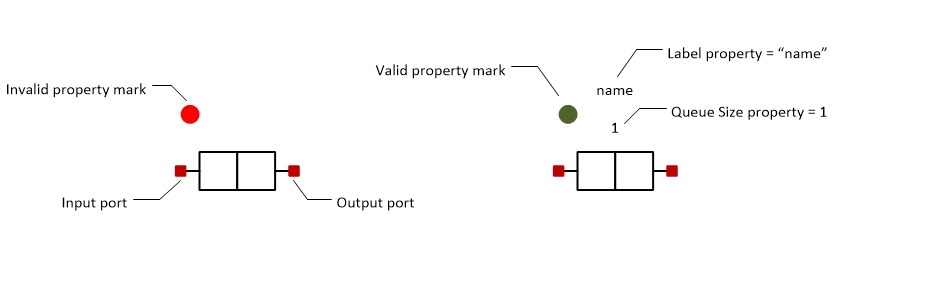
\includegraphics[width=1.0\textwidth]{queue}
The queue object its valid marker becomes green when the size property is a natural number $>$ 0. 
The queue also have a "state" property to show the verification result. 
\paragraph{Specific properties:}
\begin{itemize}
\item Size: A positive integer which represents the storage size of a queue.
\item State: Used to visualise the verification result.
\end{itemize}

\subsection{Function}

\includegraphics[width=1.0\textwidth]{function}
\paragraph{Specific properties:}
\begin{itemize}
\item Function f: is a subset of the C language, an integer which represents the packet is available through variable 'header'.
The valid marker becomes green if the  string value of the "Function f" property is not empty.

Example: ret=0;

Available operators:
\begin{itemize}
\item math operators $+,-,*,/,\%$
\item logical operators $\&\&,||,!$
\item equality operators $==,<=,>=,<,>$
\end{itemize}
\end{itemize}


\subsection{Fork}
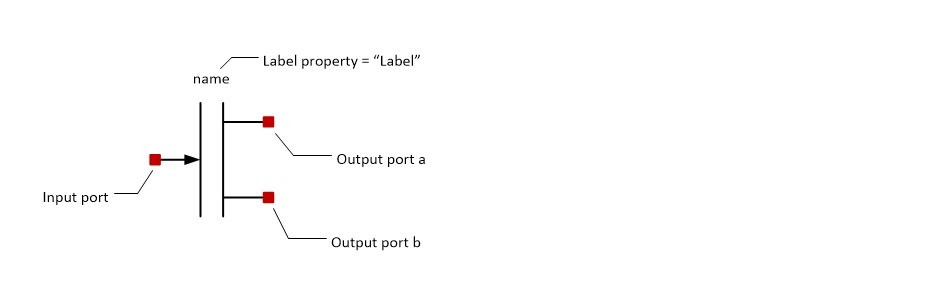
\includegraphics[width=1.0\textwidth]{fork}
A fork has no specific properties.


\subsection{Join}
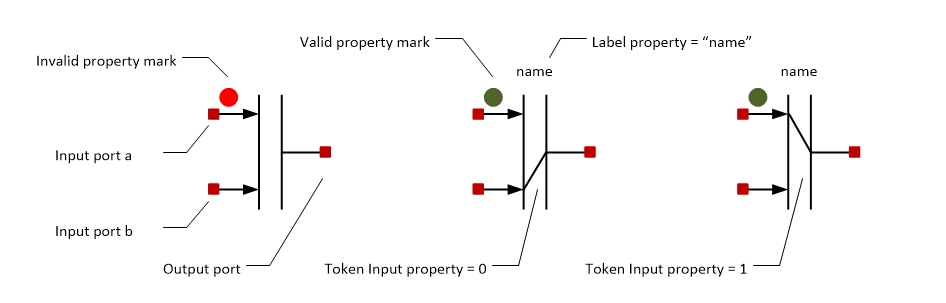
\includegraphics[width=1.0\textwidth]{join}
The join object its valid marker becomes green if the "token" property is set.
Depending on the "token" property the visualisation of the object will change.
\paragraph{Specific properties:}
\begin{itemize}
\item Token Input: "0" select input 2 while "1" selects input 1
\end{itemize}


\subsection{Switch}
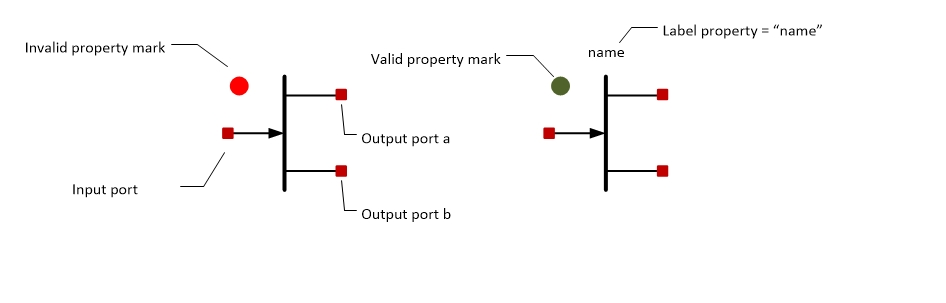
\includegraphics[width=1.0\textwidth]{switch}
\paragraph{Specific properties:}
\begin{itemize}
\item "Function s" is a subset of the C language, an integer which represents the packet is available through variable 'header'.
The valid marker becomes green if the  string value of the "Function s" property is not empty.

Example: return header == 0;

Available operators:
\begin{itemize}
\item math operators $+,-,*,/,\%$
\item logical operators $\&\&,||,!$
\item equality operators $==,<=,>=,<,>$
\end{itemize}
\end{itemize}


\subsection{Merge}
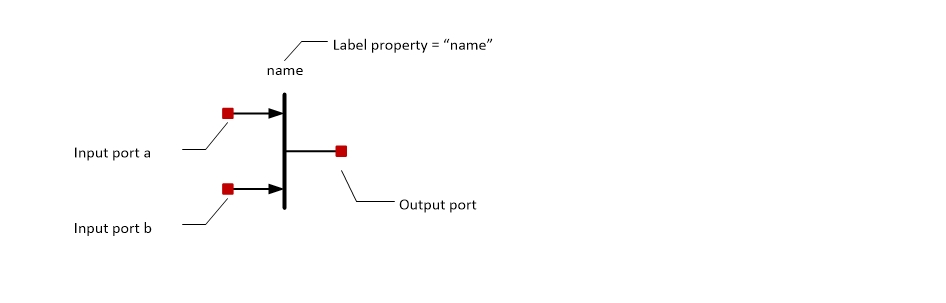
\includegraphics[width=1.0\textwidth]{merge}
A merge has no specific properties.

\subsection{Sink}
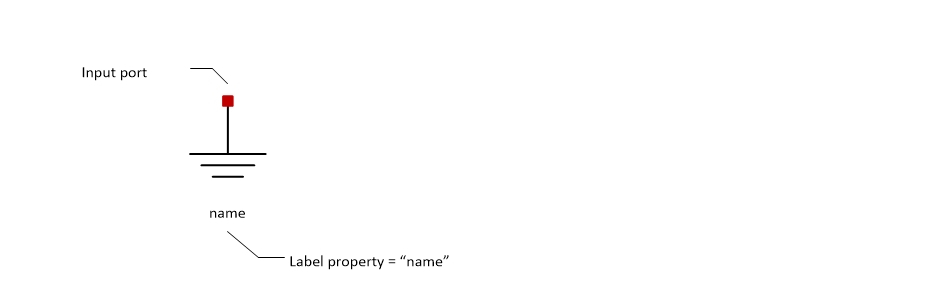
\includegraphics[width=1.0\textwidth]{sink}
A sink has no specific properties.

\subsection{Source}

\includegraphics[width=1.0\textwidth]{source}
\paragraph{Specific properties:}
\begin{itemize}
\item "Function e" insert types of packets injected at this source. The domain of all packets is available through PacketDomain.
The valid marker becomes green if the  string value of the "Function e" property is not empty.

Example: \{p in PacketDomain $|$ p $<$ 100\}
\end{itemize}


\section{Composite objects}
Because a composite object is an open network, WickedXmas provides two
additional objects to create connection points, which are in fact the resulting
ports of the composite object itself. Its purpose is meant to distinguish between a
dangling port and one that will be connected later when reusing the
composite object.

There are two kinds of connection points, the input type and the output type.
In figure~\ref{fig:CompObj} at the left you can find the graphical
representation of these objects. The properties of connection points are
the same as those for primitives and do not have any specific properties.
In the center of figure~\ref{fig:CompObj} a simple example of a
composite object being opened e.g. for editing. It is saved as file MyQ.wck
and can be reused into a larger model as shown right in figure ~\ref{fig:CompObj}.

As you can see the filename of a composite object is placed in its
body when reuse. The size of the body will be adjusted by the number
of ports, input ports left and output ports at the right side.


\begin{figure}[here]
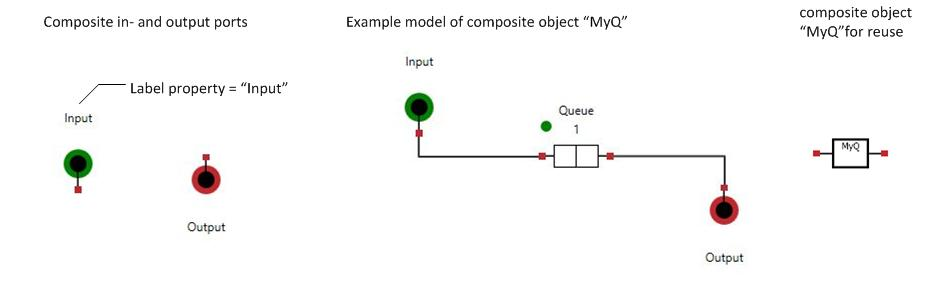
\includegraphics[width=1.0\textwidth]{CompObj}
\caption{Composite object}
\label{fig:CompObj}
\end{figure}


\newpage
\section{JSON}

An xMAS model  can be saved to disk as a file with ``wck'' extension, the file content is JSON formatted.
The WickedXmas tool uses a hierarchical structure for this and a flat structure to exchange with the verifier
tools.
An other difference between those two is the content itself, the former requires content for the
visual representation of the model while the latter only needs content related to verification.

\href{http://www.json.org/}{JSON} is a human readable lightweight scripting language for data objects similar
to XML but less complex.

The next two subsection describe those two structures.

\subsection{Hierarchical structure (wck)}
Allthough the structure of this json looks flat at first sight, the way composite objects are implemented into such
a structure unveils its hierachical structure.
The root structure of a wck JSON format has one object containing three members named:
\begin{itemize}
\item \textbf{shapes}: The value is an array containing the primitives and composite objects with their properties.
\item \textbf{connections}: This value is also an array but contains the channels or wiring between object ports.
\item \textbf{packet\_types}: This member holds fields and ranges of the packet types. 
\end{itemize}

Structure of an empty wck file:
\color{blue}
\begin{verbatim}
    {
      "shapes'': [],
      "connections'': [],
      "packet\_types'': null
    }
\end{verbatim}
\color{black}

\subsubsection{Member ``shapes''}
The ``shapes'' member its value is an array of json objects, again each object has several members,
most of these members are the same for all kind of primitives or composite objects. As you can see
in the example below the ``qSize'' value is a specific property for a queue type primitive.
So in the current WickedXmas tool there's no uniformness for this, e.g. the token property
of the join primitive is put into the ``functions'' member, so there's no reason why the qSize couldn't be
handled in a similar way. The same holds for composite objects where an extra ``fileName'' value is used to
point to the wck model file and its pathname.

There's a shape types for every primitive, two for the connection points and one for a composite object.
Additional there are also some extended primitives with 3 or 4 in or output ports.

\begin{samepage}
A ``shapes'' example of a queue type
\color{blue}
\begin{verbatim}
    {
      "qSize": 1,
      "oldShapeID": 0,
      "posX": 440,
      "posY": 184,
      "orientation": 1,
      "sizeMultiplier": 1.0,
      "type": "Queue",
      "label": "name",
      "functions": [
        "",
        ""
      ]
    }
\end{verbatim}
\color{black}
\end{samepage}

\begin{samepage}
A ``shapes'' example of a composite object type
\color{blue}
\begin{verbatim}
    {
      "fileName": "C:\\_DA_\\WickedXmas\\Models\\macro.wck",
      "oldShapeID": 11,
      "posX": 328,
      "posY": 149,
      "orientation": 1,
      "sizeMultiplier": 1.0,
      "type": "CompositeObject",
      "label": "",
      "functions": [
        "",
        ""
      ]
    }
\end{verbatim}
\color{black}
\end{samepage}

\begin{samepage}
\subsubsection{Member ``connections''}
The ``connections'' member is an array of objects and each object has four pairs, two
source pairs and two sink pairs. Each holds the identity of the shape while
the otherone holds the name of the port.
In other words an object of the connections array represents one wire or a channel.

The next json example is a ``connections'' member which forms a channel between shapeId 11 its port
``Out1'' to shapeId 12 its port ``In1''. Source means output or initiator and sink means
input or target.
\color{blue}
\begin{verbatim}
    {
      "oldSourceDesignerShapeID": 11,
      "oldSinkDesignerShapeID": 12,
      "sourceConnectorName": "Out0",
      "sinkConnectorName": "In1"
    }
    \end{verbatim}
\color{black}
\end{samepage}

\begin{samepage}
\subsubsection{Member ``packet\_types''}
The packet\_types member contains only one object and as many members as
field$-$range pairs which can be configured in the WickedXmas packet type windows.
In the example there are two packets configured.


\color{blue}
\begin{verbatim}
    {
      "type": 2,
      "test": 1
    }
\end{verbatim}
\color{black}
\end{samepage}


\subsection{Flat structure (fjson)}
The flat json structure is used to exchange the model with verify tools.
During translation from ``wck'' to ``fjson'' the xMAS model is statically
verified. If there are any errors the translation interrupts and no
fjson will be created.

In a fjson there are no composite objects anymore this because the
translator replaces the composite object with its ``wck'' content,
this until all objects has been drill down to the eight primitives.
Apart from translation, the flat json structure is of no importance
in the scope of composite objects.

Just one thing to keep in mind, the recursive reuse of a composite
object at this moment has no way to apply a condition so the
resursion stops during tranlation to a flat structure.

\newpage
\section{Similar domain example}
The company General Electric (GE) has a tool called P80i and is very similar
to the WickedXmas tool but for an other purpose.
It has been developed by several companies worldwide amongst these
were Alstom France and Converteam UK.

To tool creates VxWorks executables out of a model and is very reliable,
its used for military purpose and industries like mining, marine, oil and gas.

It has the same principle as WickedXmas, instead of writing software
in some kind of cryptic language, the user draws a model which he's
or she's familiar with and compiles it to an executable so it can be run
at a high speed on an embedded system.
So the user doesn't have to be worried about low level programming
language and its disadvantages but the benefits remain and 
above all, this way of programming is less buggy it captures
faults before they are compiled e.g. the editor prevents linking
two outputs.

The way it manages reusable software is an example as it should be.
Not the complexity gains but it forsees the basics to maintain reusable
software quite similar to well known development environements. 

Advantage of reusable software or components in P80i vs. WickedXmas:
\begin{itemize}
\item User definable representation.
\item Seperate handling instead of a mixed structure or file extension.
\item Managed as files stored into a library and not as files with absolute
paths which means a hassle when exchange designs among others.
\item Project related design, so one or more models belong to a project file
which also holds the library of reusable components and environement setup.
\end{itemize}


\begin{figure}[here]
\center
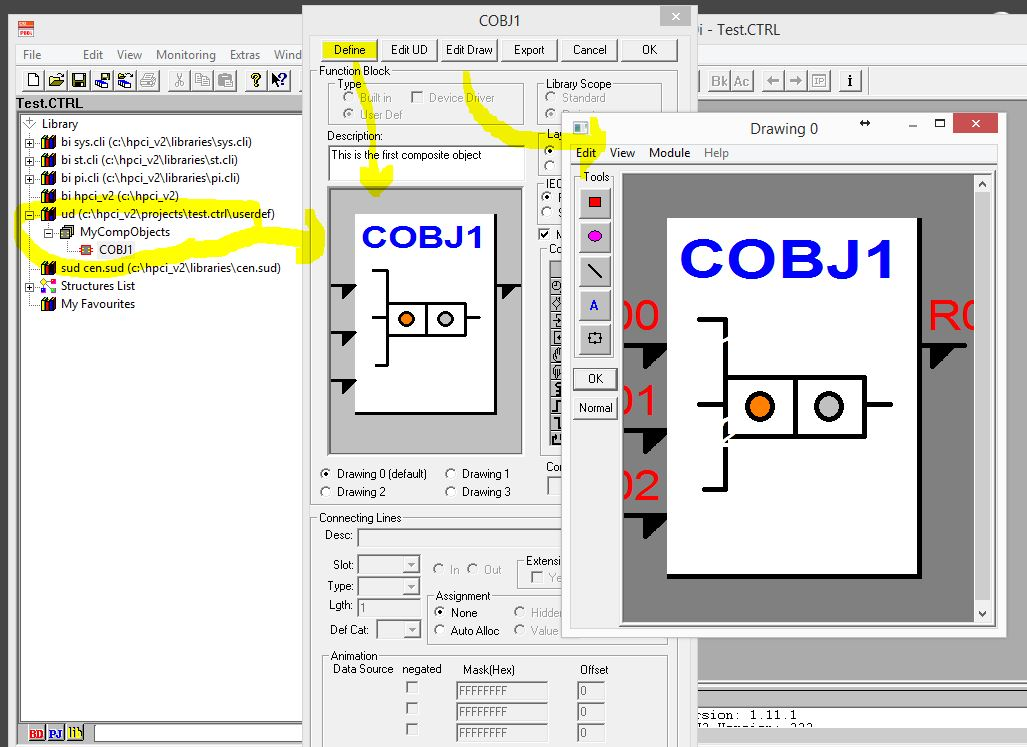
\includegraphics[width=0.50\textwidth]{p80iObjEditor.JPG}
\caption{P80i and reusable design and management}
\label{fig:p80iObjEditor}
\end{figure}
Figure~\ref{fig:p80iObjEditor} shows us how P80i manages reusable components
and how a user can define its ports and graphics.
At the left there's a tree which represents the library of selected
components for this modelling project.
A user can add new components and categorise it in the library tree, in the middle
there's a window showing us how a user can define components and at the right
how an image can be drawn on the component its body.

\begin{figure}[here]
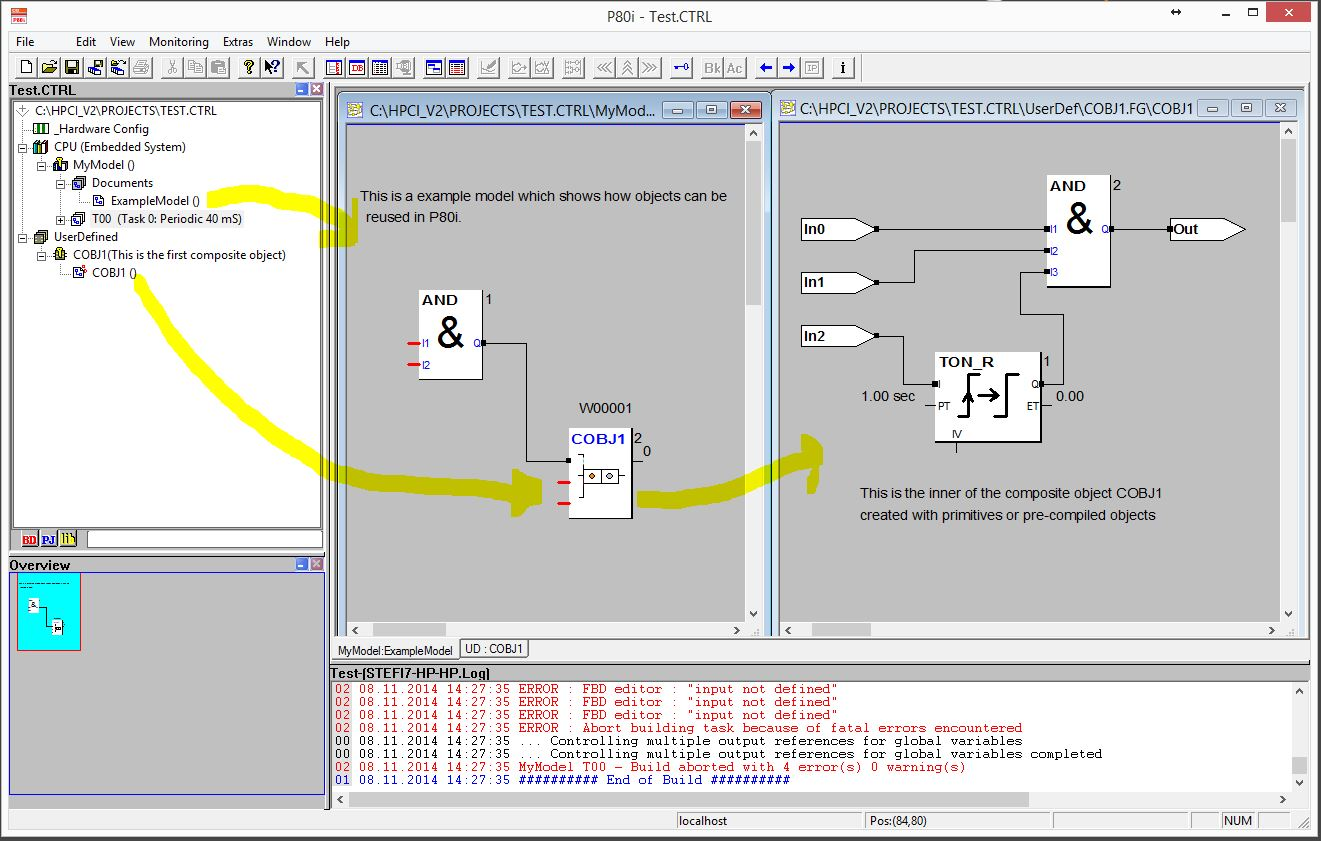
\includegraphics[width=1.0\textwidth]{p80i.JPG}
\caption{P80i showing software reuse}
\label{fig:p80i}
\end{figure}

Once this is done it need some code behind, again this is also modelling language
as shown in figure~\ref{fig:p80i}
At the left side a project tree with the composite objects in use, in the middle 
there's the model with COBJ1 as composite object and fully right the model
inside COBJ1 which can be edited just as any other model in P80i. Also
notice the in and output ports which are similar to the connection points
in WickedXmas.





\newpage
\section{Dictionary}
\begin{itemize}
	\item \textbf{WickedXmas}: Name ofthe tool used to design and analyse xMAS models.
	\item \textbf{xMAS model}:
	A model based on Intel's xMAS or e\underline{x}ecutable \underline{M}icro\underline{A}rchitectural \underline{S}pecification,
	which is ahigh level design language for communication fabrics.
	\item \textbf{Primitive Object}: The xMAS language consist of eight primitive objects which are used to create xMAS models.
	Primitive objects are hard coded.
	\item \textbf{Composite Object}: A composite object which can be made of primitives and composite objects.
	It is also known as a open xMAS model, macro or combinatorial object.
	\item \textbf{Channel}: A connection between an input and output port.
	\item \textbf{Port}: Each object has one or more ports to create a channel, there are initiator and target ports.
	\item \textbf{Connector}: see port.
	\item \textbf{Initiator}: An output port.
	\item \textbf{Target}: An input port.
	\item \textbf{Wire}: A graphical representation of a channel.
	\item \textbf{Open xMAS network}: see Composite object.
	\item \textbf{Macro or macro block}: see Composite object.
	\item \textbf{Combinatorial object}: see Composite object.
	\item \textbf{Connection point}: Object to create a port for a composite object.
	\item \textbf{Configuration}: Represents the current state of a model which means the occupation of queues.
	\item \textbf{wck}: File extension of an xMAS model and contains hierarchical structured JSON.
	\item \textbf{JSON}: \underline{J}avascript \underline{O}bject \underline{N}otation is a readable data file format comparable to XML.
	\item \textbf{fjson}: File extension of an xMAS model and contains flat structured JSON.
	\item \textbf{Sink (wck)}: see target. 
	\item \textbf{Source (wck)}: see initiator.
	\item \textbf{Message type}: Response (0) or request (1) used to setup packet type and called range.
\end{itemize}


\newpage
\section{References}
\begin{itemize}
	\item \href{http://www.json.org/}{JSON}
\end{itemize}

\end{document}